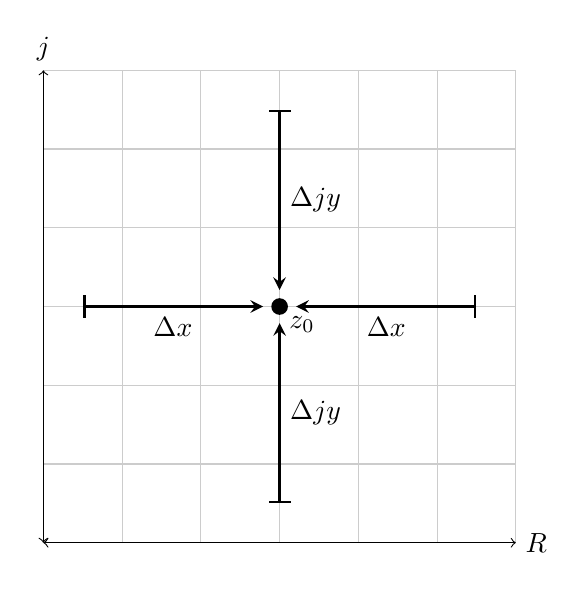
\begin{tikzpicture}
    \draw[thin,gray!40] (0,0) grid (6,6);
    \draw[<->] (0,0)--(6,0) node[right] {$R$};
    \draw[<->] (0,0)--(0,6) node[above]{$j$};

    \coordinate (a) at (3,3);
    \coordinate (b) at (2.707,2.707);
    
    \path[fill=black] (a) circle(3pt) node[anchor=north west]{$z_0$};
    \draw[line width=1pt,black,|-stealth](0.5,3)--(2.79,3) node[midway, below]{$\Delta x$};
    \draw[line width=1pt,black,|-stealth](5.5,3)--(3.21,3) node[midway, below]{$\Delta x$};
    \draw[line width=1pt,black,|-stealth](3,5.5)--(3,3.21) node[midway, right]{$\Delta jy$};
    \draw[line width=1pt,black,|-stealth](3,0.5)--(3,2.79) node[midway, right]{$\Delta jy$};
    

\end{tikzpicture}
\caption*{Plateo genérico de un limite en 4 direcciones}